In the work of \cite{marston2006evaluation}, the author wanted to test a prototype developed in previous researches on the street and in a park with a blind user. This experiment would also compare two differente guidance display, one based on haptics transmission and another based on sounds.

8 BVI participants attended the experiment, that was divided in one training set and two test sites. The first was in a busy block which had a variety of street furniture, parked bicycles and people and the participant need to pass through 4 waypoints for a total of 244m. The second site was inside a park, with paths made of concrete, crushed gravel and paver blocks, with 7 waypoint for a total of 187m. Each participant did each route with both guidances displays.

The researches collected the time to collect all waypoints, the errors made, the distance travelled and the percentage of the total time that the users accessed the guidance device. All participants were able to complete all routes and collect all waypoints with both devices. This shows that they were able to be guided by new sound or haptic devices. The mean time to collect all he waypoints using the sound device was lower than with the haptic device, as show in the Figure \ref{fig:evaluation_mean_time}. This Figure shows a standardize time made based on the time that two researchers took to complete the route, both of them blindfolded and with a cane, but already had made the same route many times before and during the experiment.

%\begin{figure}[htbp]
%    \centering
%    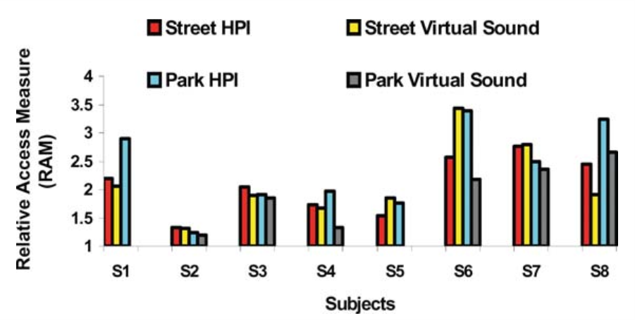
\includegraphics[width = \linewidth]{Revisao/Evaluation Spatial Display/Evaluation mean time.png}
%    \caption{Standardize mean completion time for each subject with each device in each route \cite{marston2006evaluation}.}
%    \label{fig:evaluation_mean_time}
%\end{figure}

\begin{figure}[htbp]
    \centering    
    \tikzstyle{barraHPIRua} = [fill = cor1]
    \tikzstyle{barraSomRua} = [fill = cor2]
    \tikzstyle{barraHPIParque} = [fill = cor3]
    \tikzstyle{barraSomParque} = [fill = cor4]
    \tikzstyle{legenda} = [fill = white, line width = 0.25mm]
    \tikzstyle{--} = [line width = 0.25mm]
    
    \resizebox{\linewidth}{!}{
    \begin{tikzpicture}[node distance=0cm]
        \centering    
        % Fundo do gráfico
        \renewcommand{\tamX}{16.0cm}
        \renewcommand{\tamY}{6.0cm}
        
        \node (origin) {};
        \node (endX) [xshift = \tamX] {};
        \node (endY) [yshift = \tamY] {};
        \node (endXY) [above of = endX, yshift = \tamY] {};
        
        %Título
        \node (titulo) [xshift = \tamX*0.5, yshift = \tamY + 1cm] {};
        \draw[--] (origin.west) node[anchor = east]{ 1} to (endX.center) node[anchor = north, xshift = -\tamX*0.5, yshift = -1.0cm]{\textbf{\Large Subjects}};
        \draw[--] (origin.south) to (endY.center) 
        node(eixoY)[anchor = east, xshift = -2.5cm, yshift = 0.5cm, rotate = 90]{\textbf{\Large Relative Access Measure}}
        node[right of = eixoY, anchor = west, xshift = 1.0cm, yshift = -0.75cm, rotate = 90]{\textbf{\Large (RAM)}};
        \draw[--] (endX.center) to (endXY.center);
        
       \foreach \r/\n in {1/1.5, 2/2.0, 3/2.5, 4/3.0, 5/3.5, 6/4.0}
        {
            \draw [--] (-0.15,1cm*\r) node[anchor = east]{\n} to (\tamX,1cm*\r);
        }
        
        \renewcommand{\largX}{0.25}
        \renewcommand{\altY}{0}
        
        \renewcommand{\distX}{0.5}
        %S1
        \draw[barraHPIRua] (\distX,0) rectangle ++(\largX,2.25);
        \draw[barraSomRua] (\distX+\largX,0) node[xshift = \largX*1cm, yshift = -0.5cm]{\textbf{\Large S1}} rectangle ++(\largX,2.1);
        \draw[barraHPIParque] (\distX+2*\largX,0) rectangle ++(\largX,3.9);
        \draw[barraSomParque] (\distX+3*\largX,0) rectangle ++(\largX,0);
        \draw[--] (\distX+6*\largX,0) to ++(0,-0.2);
        
        \renewcommand{\distX}{2.5}
        %S2
        \draw[barraHPIRua] (\distX,0) rectangle ++(\largX,0.6);
        \draw[barraSomRua] (\distX+\largX,0) node[xshift = \largX*1cm, yshift = -0.5cm]{\textbf{\Large S2}} rectangle ++(\largX,0.5);
        \draw[barraHPIParque] (\distX+2*\largX,0) rectangle ++(\largX,0.4);
        \draw[barraSomParque] (\distX+3*\largX,0) rectangle ++(\largX,0.3);
        \draw[--] (\distX+6*\largX,0) to ++(0,-0.2);
        
        \renewcommand{\distX}{4.5}
        %S3
        \draw[barraHPIRua] (\distX,0) rectangle ++(\largX,2.1);
        \draw[barraSomRua] (\distX+\largX,0) node[xshift = \largX*1cm, yshift = -0.5cm]{\textbf{\Large S3}} rectangle ++(\largX,1.8);
        \draw[barraHPIParque] (\distX+2*\largX,0) rectangle ++(\largX,1.9);
        \draw[barraSomParque] (\distX+3*\largX,0) rectangle ++(\largX,1.7);
        \draw[--] (\distX+6*\largX,0) to ++(0,-0.2);
        
        \renewcommand{\distX}{6.5}
        %S4
        \draw[barraHPIRua] (\distX,0) rectangle ++(\largX,1.6);
        \draw[barraSomRua] (\distX+\largX,0) node[xshift = \largX*1cm, yshift = -0.5cm]{\textbf{\Large S4}} rectangle ++(\largX,1.5);
        \draw[barraHPIParque] (\distX+2*\largX,0) rectangle ++(\largX,2.0);
        \draw[barraSomParque] (\distX+3*\largX,0) rectangle ++(\largX,0.7);
        \draw[--] (\distX+6*\largX,0) to ++(0,-0.2);
        
        \renewcommand{\distX}{8.5}
        %S5
        \draw[barraHPIRua] (\distX,0) rectangle ++(\largX,1.1);
        \draw[barraSomRua] (\distX+\largX,0) node[xshift = \largX*1cm, yshift = -0.5cm]{\textbf{\Large S5}} rectangle ++(\largX,1.7);
        \draw[barraHPIParque] (\distX+2*\largX,0) rectangle ++(\largX,1.6);
        \draw[barraSomParque] (\distX+3*\largX,0) rectangle ++(\largX,0);
        \draw[--] (\distX+6*\largX,0) to ++(0,-0.2);
        
        \renewcommand{\distX}{10.5}
        %S6
        \draw[barraHPIRua] (\distX,0) rectangle ++(\largX,3.1);
        \draw[barraSomRua] (\distX+\largX,0) node[xshift = \largX*1cm, yshift = -0.5cm]{\textbf{\Large S6}} rectangle ++(\largX,4.9);
        \draw[barraHPIParque] (\distX+2*\largX,0) rectangle ++(\largX,4.8);
        \draw[barraSomParque] (\distX+3*\largX,0) rectangle ++(\largX,2.4);
        \draw[--] (\distX+6*\largX,0) to ++(0,-0.2);
        
        \renewcommand{\distX}{12.5}
        %S7
        \draw[barraHPIRua] (\distX,0) rectangle ++(\largX,3.5);
        \draw[barraSomRua] (\distX+\largX,0) node[xshift = \largX*1cm, yshift = -0.5cm]{\textbf{\Large S7}} rectangle ++(\largX,3.6);
        \draw[barraHPIParque] (\distX+2*\largX,0) rectangle ++(\largX,3.0);
        \draw[barraSomParque] (\distX+3*\largX,0) rectangle ++(\largX,2.8);
        \draw[--] (\distX+6*\largX,0) to ++(0,-0.2);
        
        \renewcommand{\distX}{14.5}
        %S8
        \draw[barraHPIRua] (\distX,0) rectangle ++(\largX,2.9);
        \draw[barraSomRua] (\distX+\largX,0) node[xshift = \largX*1cm, yshift = -0.5cm]{\textbf{\Large S8}} rectangle ++(\largX,1.8);
        \draw[barraHPIParque] (\distX+2*\largX,0) rectangle ++(\largX,4.5);
        \draw[barraSomParque] (\distX+3*\largX,0) rectangle ++(\largX,3.2);
        \draw[--] (\distX+6*\largX,0) to ++(0,-0.2);
        
        %Legenda
        \draw[legenda] (\tamX-6.0cm,\tamY-0.75cm) rectangle ++(6.5cm,3.25cm);
        \draw[barraHPIRua] (\tamX-5.75cm,\tamY+2.0cm) rectangle ++(0.25cm,0.25cm) 
        node[anchor = west, xshift = 0.15cm, yshift = -0.15cm]{\Large Street HPI};
        \draw[barraSomRua] (\tamX-5.75cm,\tamY+1.25cm) rectangle ++(0.25cm,0.25cm) 
        node[anchor = west, xshift = 0.15cm, yshift = -0.15cm]{\Large Street Virtual Sound};
        \draw[barraHPIParque] (\tamX-5.75cm,\tamY+0.5cm) rectangle ++(0.25cm,0.25cm) 
        node[anchor = west, xshift = 0.15cm, yshift = -0.15cm]{\Large Park HPI};
        \draw[barraSomParque] (\tamX-5.75cm,\tamY-0.25cm) rectangle ++(0.25cm,0.25cm) 
        node[anchor = west, xshift = 0.15cm, yshift = -0.15cm]{\Large Park Virtual Sound};
        
    \end{tikzpicture}
    }
    \caption{Standardize mean completion time for each subject with each device in each route (Adapted from \citeonline{marston2006evaluation}).}
    \label{fig:evaluation_mean_time}
\end{figure}

Another finding from this work is about the use haptic device the cause some strain at the arm and was less acceptable as compaired to the sound device, that required no use of the arms.

This study was relevant for current work because it also compares the same types of guidance devices. The participants were asked to score both devices in three questions from 1 = very unacceptable to 5 = very acceptable. These scores are presented in the Table \ref{tab:evaluation_table}. As said above, the participants were able to perform the full experiment with both devices, but there seems to be a preference for the sound-based device.

\begin{table}[htbp]
    \centering
    \caption{Scores of the device}
    \label{tab:evaluation_table}
    \begin{tabular}{|l|l|l|l|l|}
        \hline
        \multirow{2}{*}{\textbf{Statement}} &
        \multirow{2}{*}{\textbf{\begin{tabular}[c]{@{}l@{}}Haptic device's\\ mean score \end{tabular}}} & \multirow{2}{*}{\textbf{SD}} &
        \multirow{2}{*}{\textbf{\begin{tabular}[c]{@{}l@{}}Sound device's \\ mean score\end{tabular}}} & 
        \multirow{2}{*}{\textbf{SD}} \\
        &&&& \\ \hline
        Precision of the directiona information & 4.0 & 0    & 4.1 & 0.83 \\ \hline
        Personal safety while using the device  & 4.1 & 0.35 & 4.0 & 0.76 \\ \hline
        Ease of use                             & 3.5 & 0.53 & 4.6 & 0.52 \\ \hline
    \end{tabular}
\end{table}

But what about being able to use both devices? That's one of the questions that the experiment of this master's thesis aims to answer.